% Have TexShop run the whole thing
%!TEX TS-program = pdflatexmk

%\documentclass[handout,18pt]{beamer}
\documentclass[18pt]{beamer}
\usetheme{Madrid}

\usepackage{hyperref}
% \usepackage{ulem,cite,caption,amsmath,graphicx}
\usepackage{float}
\usepackage{listings}
\usepackage{paralist}
% \usepackage[htt]{hyphenat}
% \usepackage{enumerate}
% \usepackage{enumitem}
\usepackage{threeparttable}
\usepackage{float}
\usepackage{verbatim}
% \setlist{nolistsep}

\usepackage{url}

% New float environment
% \newfloat{listing}{tbphH}{lopbl}
% \floatname{listing}{Listing}
% \newsubfloat{listing}

\definecolor{listcomment}{rgb}{0.0,0.5,0.0}
\definecolor{listkeyword}{rgb}{0.0,0.0,0.5}
\definecolor{listnumbers}{gray}{0.65}
\definecolor{listlightgray}{gray}{0.955}
\definecolor{listwhite}{gray}{1.0}

% Now can put escape sequences inside listings.
\lstset{escapeinside={(*}{*)}}
\lstdefinelanguage{Lua}
  {morecomment=[l]{--},
}

 \newcommand{\lstcpp}
 {
\lstset{frame = tb,
    framerule = 0.25pt,
    belowcaptionskip = 8pt,
    float,
    %fontadjust,
    backgroundcolor={\color{listlightgray}},
    basicstyle = {\ttfamily\footnotesize},
    keywordstyle = {\ttfamily\color{listkeyword}\textbf},
    identifierstyle = {\ttfamily},
    commentstyle = {\ttfamily\color{listcomment}\textit},
    stringstyle = {\ttfamily},
    showstringspaces = false,
    showtabs = false,
    % numbers = left,
    numbersep = 2pt,
    numberstyle={\ttfamily\color{listnumbers}},
    tabsize = 2,
    language=[ANSI]C++,
    floatplacement=!h
  }
}
 \newcommand{\lstjava}
 {
\lstset{frame = tb,
    framerule = 0.25pt,
    belowcaptionskip = 8pt,
    float,
    %fontadjust,
    backgroundcolor={\color{listlightgray}},
    basicstyle = {\ttfamily\footnotesize},
    keywordstyle = {\ttfamily\color{listkeyword}\textbf},
    identifierstyle = {\ttfamily},
    commentstyle = {\ttfamily\color{listcomment}\textit},
    stringstyle = {\ttfamily},
    showstringspaces = false,
    showtabs = false,
    % numbers = left,
    numbersep = 2pt,
    numberstyle={\ttfamily\color{listnumbers}},
    tabsize = 2,
    language=Java,
    floatplacement=!h
  }
}
 \newcommand{\lstmatlab}
 {
\lstset{frame = tb,
    framerule = 0.25pt,
    belowcaptionskip = 8pt,
    float,
    fontadjust,
    backgroundcolor={\color{listlightgray}},
    basicstyle = {\ttfamily\footnotesize},
    keywordstyle = {\ttfamily\color{listkeyword}\textbf},
    identifierstyle = {\ttfamily},
    commentstyle = {\ttfamily\color{listcomment}\textit},
    stringstyle = {\ttfamily},
    showstringspaces = false,
    showtabs = false,
    % numbers = left,
    numbersep = 6pt,
    numberstyle={\ttfamily\color{listnumbers}},
    tabsize = 2,
    language=Matlab,
    floatplacement=!h
  }
}

 \newcommand{\lstlua}
 {
\lstset{frame = tb,
    framerule = 0.25pt,
    belowcaptionskip = 8pt,
    float,
    fontadjust,
    backgroundcolor={\color{listlightgray}},
    basicstyle = {\ttfamily\footnotesize},
    keywordstyle = {\ttfamily\color{listkeyword}\textbf},
    identifierstyle = {\ttfamily},
    commentstyle = {\ttfamily\color{listcomment}\textit},
    stringstyle = {\ttfamily},
    showstringspaces = false,
    showtabs = false,
    % numbers = left,
    numbersep = 6pt,
    numberstyle={\ttfamily\color{listnumbers}},
    tabsize = 2,
    language=Lua,
    floatplacement=!h
  }
}

 \newcommand{\lstpython}
 {
\lstset{frame = tb,
    framerule = 0.25pt,
    belowcaptionskip = 8pt,
    float,
    fontadjust,
    backgroundcolor={\color{listlightgray}},
    basicstyle = {\ttfamily\footnotesize},
    keywordstyle = {\ttfamily\color{listkeyword}\textbf},
    identifierstyle = {\ttfamily},
    commentstyle = {\ttfamily\color{listcomment}\textit},
    stringstyle = {\ttfamily},
    showstringspaces = false,
    showtabs = false,
    % numbers = left,
    numbersep = 6pt,
    numberstyle={\ttfamily\color{listnumbers}},
    tabsize = 2,
    language=Python,
    floatplacement=!h
  }
}

\definecolor{listcomment}{rgb}{0.0,0.5,0.0}
\definecolor{listkeyword}{rgb}{0.0,0.0,0.5}
\definecolor{listnumbers}{gray}{0.65}
\definecolor{listlightgray}{gray}{0.955}
\definecolor{listwhite}{gray}{1.0}

\definecolor{listcomment}{rgb}{0.0,0.0,1.0}
\definecolor{listkeyword}{rgb}{0.5,0.0,0.0}
\definecolor{listidentifier}{rgb}{0.0,0.3,0.0}
\definecolor{listdirective}{rgb}{0.5,0.0,1.0}
\definecolor{liststring}{rgb}{1.0,0.0,1.0}
\definecolor{listnumbers}{gray}{0.65}
\definecolor{listlightgray}{gray}{0.955}
\definecolor{listwhite}{gray}{1.0}
\definecolor{listbackground}{rgb}{0.9,0.9,1.0}


\lstset{language=C++}
\lstset{numbers=left}
\lstset{frame=tb}
\lstset{xleftmargin=0.05\linewidth}
\lstset{backgroundcolor=\color{listbackground}}
\lstset{basicstyle=\tiny}
\lstset{keywordstyle=\color{listkeyword}\bfseries}
\lstset{identifierstyle=\color{listidentifier}}
\lstset{directivestyle=\color{listdirective}}
\lstset{commentstyle=\color{listcomment}}
\lstset{stringstyle=\ttfamily\color{liststring}}
\lstset{showstringspaces=false}

\newcommand{\lstlistingwithnumber}[3]{
\begin{center}
\lstinputlisting[linerange={#1-#2},firstnumber=#1,numbers=left]{#3}
\end{center}
}


\newcommand{\centeredlargetext}[3]{
{
\setbeamertemplate{navigation symbols}{}
\setbeamercolor{background canvas}{bg={#1}}
\color{#2}
\begin{frame}[plain]
\fontsize{36pt}{36pt}\selectfont
\center
\begin{center}
{#3}
\end{center}
\end{frame}
}}

\newcommand{\centeredhugetext}[3]{
{
\setbeamertemplate{navigation symbols}{}
\setbeamercolor{background canvas}{bg={#1}}
\fontsize{72pt}{72pt}\selectfont
\color{#2}
\begin{frame}[plain]
\center
\begin{center}
{#3}
\end{center}
\end{frame}
}}


\begin{document}
\title[SimpleITK - MICCAI 2011]{SimpleITK Tutorial}
\subtitle[IP for mere mortals]{Image processing for mere mortals}
\institute[Insight Software Consortium]{Insight Software Consortium}
\date[Sept 2011]{Sept 23, 2011}

\begin{frame}
\titlepage
\end{frame}

%% {
\setbeamertemplate{navigation symbols}{}
\begin{frame}[plain]
\center
\begin{center}
This presentation is copyrighted by\\
The \textbf{Insight Software Consortium}\\
\bigskip
distributed under the\\
\textbf{Creative Commons by Attribution License 3.0}\\
\url{http://creativecommons.org/licenses/by/3.0}\\
\end{center}
\end{frame}
}

\section{Introduction}

\begin{frame}
\frametitle{What this Tutorial is about}
\begin{itemize}
\item Provide working knowledge of the SimpleITK platform
\end{itemize}
\end{frame}

\begin{frame}
\frametitle{Program}

\begin{itemize}
\item Virtual Machines Preparation (10min)
\item Introduction (15min)
\item Basic Tutorials I (45min)
\item \textcolor{gray}{Short Break (10min)}
\item Basic Tutorials II (45min)
\item \textcolor{gray}{Coffee Break (30min)}
\item Intermediate Tutorials (45min)
\item \textcolor{gray}{Short Break (10min)}
\item Advanced Topics (40min)
\item Wrap-up (10min)
\end{itemize}

\end{frame}

%% \section{Virtual Machine Preparation}

\centeredlargetext{white}{black}{
Virtual Machine Preparation
}

\begin{frame}
\frametitle{Virtual Machines Preparation}
\begin{itemize}
\item Get DVD / USB Memory Stick
\item Install VirtualBox from it
\item Import the VirtualMachine file
\item Boot the Virtual Machine
\item Get familiar
\end{itemize}
\end{frame}

\begin{frame}
\frametitle{Media Content}
\framesubtitle{Directories and Files}
\begin{itemize}
\item VirtualBoxInstallers
\begin{itemize}
\item VirtualBox-4.0.8-71778-OSX.dmg (Mac)
\item VirtualBox-4.0.8-71778-Win.exe (Windows)
\item (Ubuntu Linux)
\begin{itemize}
\item virtualbox-4.0\_4.0.8-71778~Ubuntu~lucid\_amd64.deb
\item virtualbox-4.0\_4.0.8-71778~Ubuntu~lucid\_i386.deb
\item virtualbox-4.0\_4.0.8-71778~Ubuntu~maverick\_amd64.deb
\item virtualbox-4.0\_4.0.8-71778~Ubuntu~maverick\_i386.deb
\item virtualbox-4.0\_4.0.8-71778~Ubuntu~natty\_amd64.deb
\item virtualbox-4.0\_4.0.8-71778~Ubuntu~natty\_i386.deb
\item \ldots
\end{itemize}
\end{itemize}
\item VirtualMachine
\begin{itemize}
\item  SimpleITK.ova
\end{itemize}
\end{itemize}
\end{frame}

\begin{frame}
\frametitle{Install VirtualBox}
\begin{itemize}
\item Select the installer for your platform
\item Run it
\end{itemize}
\end{frame}

\begin{frame}
\frametitle{Alternative Linux Installation}
\begin{itemize}
\item  You can also install VirtualBox by doing:
\item  sudo apt-get install virtualbox-ose-qt
\end{itemize}
\end{frame}

\begin{frame}
\frametitle{Importing the Virtual Machine}
\begin{itemize}
\item Run VirtualBox
\item In \texttt{File} Menu select \texttt{Import Appliance}
\item Provide the filename in the DVD / USB stick \texttt{VirtualMachine/SimpleITK.ova}
\item A progress bar will appear, and when it finishes you should see:
\end{itemize}
\begin{center}
  % \includegraphics[width=0.5\paperwidth]{Screenshot-VirtualBox-OSE-01.png}
\end{center}
\end{frame}


\centeredlargetext{white}{black}{
Now, on to the tutorial...
}

%% \section{Introduction}

\begin{frame}
\frametitle{Introductions}

\begin{itemize}
\item Daniel Blezek, Ph.D., Mayo Clinic
\item Luis Ib\'a\~nez, Ph.D., Kitware
\item Bradley Lowekamp, Lockheed Martin (National Library of Medicine)
\end{itemize}

\end{frame}

\begin{frame}
\frametitle{Tutorial Goals}
\begin{itemize}
\item Gentle introduction to ITK
\item Introduce SimpleITK
\item Provide hands-on experience
\item Problem solving, not direction following
\item ...but please follow directions!
\end{itemize}
\end{frame}

\begin{frame}
\frametitle{ITK Overview}
How many are familiar with ITK?
\end{frame}

\begin{frame}
\frametitle{Ever seen code like this?}
\begin{center}
\lstcpp
\lstinputlisting{Code/DiscreteGaussianFilter.cxx}
\end{center}
\end{frame}

\begin{frame}
\frametitle{What if you could write this?}
\begin{center}
\lstpython
\lstinputlisting{Code/DiscreteGaussianFilter.py}
\end{center}
\pause
We are here to tell you that you can...
\end{frame}

\begin{frame}{Goals of SimpleITK}
\begin{itemize}
\item Provide a typeless layer for ITK in C++
\item Provide wrappings in scripting languages
\item Simplify the use of ITK
\item Be an ``on-ramp'' for ITK
\end{itemize}
\end{frame}

\begin{frame}{SimpleITK Architectural Overview}
\begin{itemize}
\item Conceptually, SimpleITK is an application library built on ITK
\item Provides no functionality apart from what ITK
\item Consists of:
  \begin{itemize}
    \item Template expansion system
    \item C++ library
    \item Small SWIG definition (more details later)
    \item ``Glue'' code for several scripting languages
    \item Some language utilities
  \end{itemize}
\end{itemize}
\end{frame}

\begin{frame}{Templates in ITK}
\begin{center}
\lstcpp
\lstinputlisting{Code/ITKTemplateSample.cxx}
\end{center}
\end{frame}

\begin{frame}
\frametitle{Template Freedom}
\end{frame}

\begin{frame}
\frametitle{Programming Models}
\begin{itemize}
\item Object oriented
\item Function oriented
\end{itemize}
\end{frame}

\begin{frame}
\frametitle{Wrapping}
Transformed by SWIG
\end{frame}





% LocalWords:  SimpleITK typeless ITK

%% \section{Basic Tutorials}

\subsection{Image Basics}
\begin{frame}
\frametitle{Image Class}
\end{frame}


\subsection{Input/Output}

\begin{frame}
\frametitle{Read an image}
\end{frame}

\begin{frame}
\frametitle{Write an image}
\end{frame}

\begin{frame}
\frametitle{Display an image}
\end{frame}

\subsection{Filters}

\begin{frame}
\frametitle{Where did the pipeline go?}
\end{frame}

\begin{frame}
\frametitle{How filters work}
\end{frame}





\section{Basic Tutorials 2}

%%%%%%%%%%%%%
\subsection{Filters}

%% Break
\begin{frame}{Basic Tutorial 2}
\fontsize{36pt}{36pt}\selectfont
\center
\begin{center}
Basic Tutorial 2
\end{center}
\end{frame}

\begin{frame}{Wrapped Languages}
\fontsize{36pt}{36pt}\selectfont
\center
\begin{center}
Wrapped Languages
\end{center}
\end{frame}

\begin{frame}[fragile]
\frametitle{Wrapping Process}
\begin{center}
  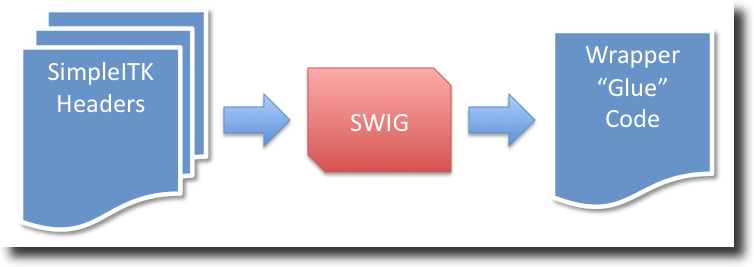
\includegraphics[width=.8\textwidth]{Images/WrappingProcess_shadow}
\end{center}
\begin{itemize}
  \item SimpleITK headers are constructed for wrapping
  \item SWIG is an open source package
  \begin{itemize}
    \item Parses C/C++ code, produces ``glue'' code
    \item Well supported, covers 10+ languages
  \end{itemize}
  \item Main languages: Python, Java, C\#
  \item Also supported: Tcl, Lua, R
\end{itemize}
\end{frame}

\begin{frame}[fragile]
\frametitle{Object Paradigm (Python)}
The paradigms translate to the wrapped languages (C++ $\rightarrow$ Python)
\lstcpp
\begin{lstlisting}
#include <SimpleITK.h>
using itk::simple;
...
// Create a smoothing filter
SmoothingRecursiveGaussianImageFilter gaussian;
// Set a parameter
gaussian.SetSigma ( 2.0 );
// "Execute" the Filter
Image blurredImage = gaussian.Execute ( image );
\end{lstlisting}
\lstpython
\begin{lstlisting}
from SimpleITK import *
# Create a smoothing filter
SmoothingRecursiveGaussianImageFilter gaussian
# Set a parameter
gaussian.SetSigma ( 2.0 );
# "Execute" the Filter
blurredImage = gaussian.Execute ( image );
\end{lstlisting}
\end{frame}

\begin{frame}[fragile]
\frametitle{Object Paradigm (Java)}
\lstjava
\begin{lstlisting}
import org.itk.simple.*;
...

// Create a smoothing filter
SmoothingRecursiveGaussianImageFilter gaussian =
      new SmoothingRecursiveGaussianImageFilter();

// Set a parameter
gaussian.SetSigma ( 2.0 );

// "Execute" the Filter
Image blurredImage = gaussian.Execute ( image );
\end{lstlisting}
\end{frame}


\begin{frame}[fragile]
\frametitle{Object Paradigm (C\#)}
\lstjava
\begin{lstlisting}
using System;
using itk.simple;
...
// Create a smoothing filter
SmoothingRecursiveGaussianImageFilter gaussian =
      new SmoothingRecursiveGaussianImageFilter();

// Set a parameter
gaussian.SetSigma ( 2.0 );

// "Execute" the Filter
Image blurredImage = gaussian.Execute ( image );
\end{lstlisting}
\end{frame}


\begin{frame}{Note on the Tutorial}
\begin{itemize}
  \item Most examples will be Python
  \item Obvious translation to other languages
  \item C++ usage (generally) obvious
\end{itemize}
\end{frame}

\subsection{Example}
\begin{frame}{Hands On}
\fontsize{36pt}{36pt}\selectfont
\center
\begin{center}
Hands On
\end{center}
\vspace{20pt}
\begin{center}
\fontsize{11pt}{11pt}\selectfont
\texttt{Examples/BasicTutorial2/Filters.py}
\end{center}
\end{frame}

\begin{frame}[fragile]
\frametitle{What just happened?}
\lstpython
\begin{lstlisting}
# Simple smoothing
smooth = sitk.SmoothingRecursiveGaussian ( image, 2.0 )
sitk.Show ( sitk.Subtract ( image, smooth ) )
...
RuntimeError: Exception thrown in SimpleITK Subtract: ...
sitk::ERROR: Both images for SubtractImageFilter don't match type or dimension!
...
\end{lstlisting}

\begin{itemize}
  \item The output of SmoothingRecursiveGaussian is of type float
  \item The input image is signed short
  \item Most SimpleITK filters with 2 inputs require the same type
  \item Let's fix the problem
\end{itemize}

\end{frame}

\begin{frame}[fragile]
\frametitle{Introducing Cast}
\lstpython
\begin{lstlisting}
# Much better
print "Before: ", smooth.GetPixelIDTypeAsString()
smooth = sitk.Cast ( smooth, image.GetPixelIDValue() )
print "After: ", smooth.GetPixelIDTypeAsString()
sitk.Show ( sitk.Subtract ( image, smooth ), "DiffWithGaussian" )
\end{lstlisting}
Back to iPython (\texttt{Examples/BasicTutorial2/Filters.py})
\end{frame}

%% Morphology
\subsection{Morphology}

\begin{frame}{Morphology}
\fontsize{36pt}{36pt}\selectfont
\center
\begin{center}
Morphology
\end{center}
\vspace{20pt}
\begin{center}
\fontsize{11pt}{11pt}\selectfont
\texttt{Examples/BasicTutorial2/Morphology.py}
\end{center}
\end{frame}

\begin{frame}[fragile]
\frametitle{Operators}

\begin{columns}[c]

\column{0.25\textwidth}
\begin{center}
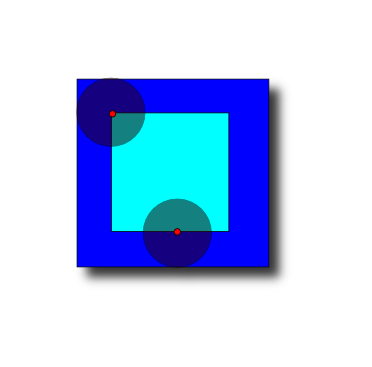
\includegraphics[width=1\textwidth]{Images/Erosion_shadow} \\
Erosion
\end{center}

\column{0.25\textwidth}
\begin{center}
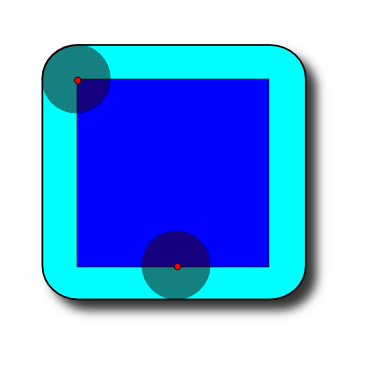
\includegraphics[width=1\textwidth]{Images/Dilation_shadow} \\
Dilation
\end{center}

\column{0.25\textwidth}
\begin{center}
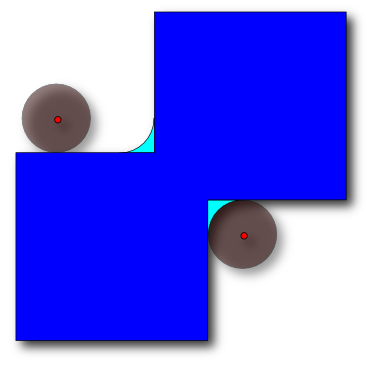
\includegraphics[width=1\textwidth]{Images/Closing_shadow} \\
Closing
\end{center}

\column{0.25\textwidth}
\begin{center}
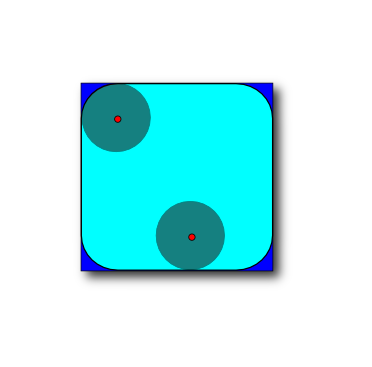
\includegraphics[width=1\textwidth]{Images/Opening_shadow} \\
Opening
\end{center}
\end{columns}
\vspace{12pt}
Images from \url{http://en.wikipedia.org/wiki/Mathematical_morphology}
\end{frame}

\begin{frame}{Morphology in Action}
\center
\begin{center}
Back to iPython (\texttt{Examples/BasicTutorial2/Morphology.py})
\end{center}
\end{frame}


\subsection{Label Maps}

%% Label maps
\begin{frame}{Label Maps}
\fontsize{36pt}{36pt}\selectfont
\center
\begin{center}
Label Maps
\end{center}
\end{frame}

%% Break
\begin{frame}{Break}
\fontsize{36pt}{36pt}\selectfont
\center
\begin{center}
Let's take a break
\end{center}
\end{frame}


\section{Interactive sessions}

%
% The idea I am going with for this section is to introduce a few
% filters. Give the audience a suggested image to load, to experiment
% with the filters as they are being describe. Then pose a problem
% which uses the prior filters for them to solve.
%

\begin{frame}
\frametitle{True utility of SimpleITK}
\begin{itemize}
\item Interacting with data
\end{itemize}
\end{frame}

\subsection{Threshold-based Segmentation}

\begin{frame}[fragile]
\frametitle{Data To Interact With}
\lstpython
\begin{lstlisting}
# Read image, using ipython's tab auto-complete
image = sitk.ReadImage( ``~/SimpleITK-MICCAI-2011-Tutorial/iasem-cells.nrrd'' )

# Get familiar with the image
print image
...
sitk.Show( image )
\end{lstlisting}
\begin{itemize}
  \item ``Dual-Beam'' or Ion-Abrasion Scanning Electron Microscope
  \item Heavily pre-proccessed
  \item  X-Z cross-section of a 3D volume
\end{itemize}
\end{frame}

\begin{frame}{Image Masks or Binary Images}
Image masks are just SimpleITK Images
\begin{itemize}
  \item Follow some conventions
  \item Pixel type of \texttt{uint8\_t}
  \item 0-value is background, 1-value being the foreground
  \item Masks are used for output of thresholding, binary morphology, etc\dots
  \item The 1-value was choosen to each of computataion with operators
  \item If a mask needs to be directly shown, multiply by 255
\end{itemize}
\end{frame}



\begin{frame}[fragile]
\frametitle{Threshold-based Segmentation}

\begin{itemize}
  \item {\bf Threshold}\\
    \small
    $ Output(x_i) =
    \begin{cases} Input(x_i) &\text{if $Lower \leq x_i \leq Upper$;}  \\
      OutsideValue            &\text{otherwise.}
    \end{cases} $
    \normalsize
  \item {\bf BinaryThreshold}\\
    \small
    $ Output(x_i) =
    \begin{cases} InsideValue &\text{if $LowerThreshold \leq x_i \leq UpperThreshold$;}  \\
      OutsideValue            &\text{otherwise.}
    \end{cases} $
    \normalsize
  \item {\bf OtsuThreshold} - Automatic Threshold values based on minimizing intra-class variance.
  \item {\bf DoubleThreshold} - A morphology based filters. Uses two sets of thresholds.
\end{itemize}

\lstpython
\begin{lstlisting}
# quick visualizations of masked image
sitk.Show( image * mask )
sitk.Show( .5*image*~mask+image*mask )
\end{lstlisting}

\end{frame}


\begin{frame}{Advanced Geodesic Morphology}

\begin{itemize}
  \item {\bf BinaryOpeningByReconstruction} - Removes binary elements which are smaller than the structuring element.
  \item {\bf BinaryClosingByReconstruction} - Fills binary holes which are smaller then the structuring element.
  \item {\bf BinaryFillHole} - Fills all holes in image.
  \item {\bf BinaryGrindPeak} - Removes all binary elements not connected to boarder.
\end{itemize}

\end{frame}

\begin{frame}{Change Border Problem}

After registration a border of the average intensity was added. Change this border to 0.

\end{frame}

\begin{frame}{Change Border Solution}
\end{frame}

\subsection{Numpy Interface}
\begin{frame}[fragile]
\frametitle{SimpleITK with Numpy}

Functions to interface SimpleITK with numpy:

\lstpython
\begin{lstlisting}
def GetArrayFromImage(image):
    """Get a numpy array from a SimpleITK Image."""

def GetImageFromArray( arr ):
    """Get a SimpleITK Image from a numpy array."""
\end{lstlisting}
\begin{itemize}
  \item Both of these methods do a deep copy of the image
  \item Ensures safety, bypassing error-prone memory issues
\end{itemize}

\end{frame}

%
% Begin Section For Hans
%

\subsection{Image Measurements}
\begin{frame}{Image Statistics}
\end{frame}

\begin{frame}{Label Statistics}
\end{frame}


\begin{frame}{Statistics Problem}
\end{frame}

\begin{frame}{Statistics Solution}
\end{frame}


%
% End Section For Hans
%

\subsection{Feature Detection}
\begin{frame}{Edge Detection}
\end{frame}

\begin{frame}{Image Derivatives}
\end{frame}

\begin{frame}{Zero Crossing}
\end{frame}


\begin{frame}{Ridge Detection Problem}
\end{frame}

\begin{frame}{Ridge Detection Solution}
\end{frame}





\section{Advanced Topics}
\begin{frame}{Advanced Topics}
\fontsize{36pt}{36pt}\selectfont
\center
\begin{center}
Advanced Topics
\end{center}
\end{frame}

\begin{frame}[fragile]
\frametitle{Building SimpleITK in 5 Easy Commands}
\small
\begin{verbatim}
git clone --recursive https://github.com/SimpleITK/SimpleITK
( cd SimpleITK && git checkout va01 )
mkdir SimpleITK-build && cd SimpleITK-build
cmake ../SimpleITK/SuperBuild
make -j 5
\end{verbatim}
\normalsize
\end{frame}

\begin{frame}[fragile]
\frametitle{More complete version}
\begin{itemize}
  \item Check out the code from GitHub (\url{https://github.com/SimpleITK/SimpleITK})
  \item Run CMake (\url{http://www.cmake.org/}) using SimpleITK/SuperBuild as the source directory
  \item Build using your favorite compiler
\end{itemize}
\end{frame}

\begin{frame}[fragile]
\frametitle{Supported Platforms}
\begin{itemize}
  \item Windows: Visual Studio 10
  \item Windows: Visual Studio 9 (Requires TR1 service pack)
  \item Mac OSX: gcc 4.x
  \item Linux: gcc 4.x
\end{itemize}
\end{frame}

\begin{frame}{SimpleITK Architecture}
\fontsize{36pt}{36pt}\selectfont
\center
\begin{center}
SimpleITK Architecture
\end{center}
\end{frame}

\begin{frame}[fragile]
\frametitle{Filter Anatomy}
\begin{center}
  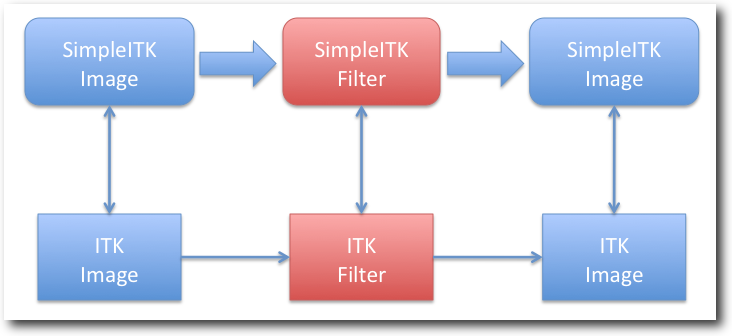
\includegraphics[width=.8\textwidth]{Images/FilterOverview_shadow}
\end{center}
\begin{itemize}
  \item SimpleITK filters create ITK filters
  \item Templated based on input type
  \item Output type is usually the same as input type
  \item Instantiated for many possible image types
\end{itemize}
\end{frame}

\begin{frame}[fragile]
\frametitle{Image and Filter Types}
\begin{columns}
  \begin{column}{0.5\textwidth}
    \begin{itemize}
      \item Dimensions
      \begin{itemize}
        \item 2 dimensional
        \item 3 dimensional
      \end{itemize}
      \item Scalar types
      \begin{itemize}
        \item $int8\_t$
        \item $uint8\_t$
        \item $int16\_t$
        \item $uint16\_t$
        \item $int32\_t$
        \item $uint32\_t$
        \item $float$
        \item $double$
        \item $std::complex< float >$
        \item $std::complex< double >$
      \end{itemize}
    \end{itemize}
  \end{column}

  \begin{column}{0.5\textwidth}
     \begin{itemize}
       \item Vector Types
       \begin{itemize}
         \item $int8\_t$
         \item $uint8\_t$
         \item $int16\_t$
         \item $uint16\_t$
         \item $int32\_t$
         \item $uint32\_t$
         \item $float$
         \item $double$
       \end{itemize}
       \item Label Types
       \begin{itemize}
         \item $uint8\_t$
         \item $uint16\_t$
         \item $uint32\_t$
       \end{itemize}
    \end{itemize}
  \end{column}
\end{columns}
\end{frame}

\begin{frame}[fragile]
\frametitle{Filter Anatomy}
\begin{center}
  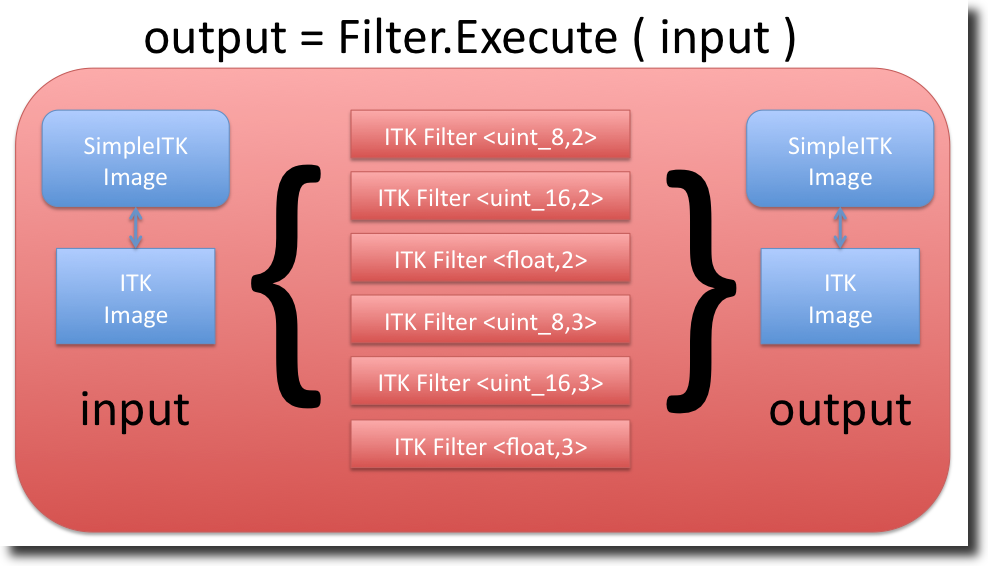
\includegraphics[width=.8\textwidth]{Images/FilterInternals_shadow}
\end{center}
\begin{itemize}
  \item Filter interrogates $input$
  \item Instantiates proper ITK filter
  \item Executes ITK filter
  \item Constructs $output$ from ITK image
\end{itemize}
\end{frame}

\subsection{Using Filters}
\begin{frame}{Using Filters}
\fontsize{36pt}{36pt}\selectfont
\center
\begin{center}
Using Filters
\end{center}
\end{frame}

\begin{frame}[fragile]
\frametitle{Object Paradigm (C++)}
\lstcpp
\begin{lstlisting}
#include <SimpleITK.h>
namespace sitk = itk::simple;
...
// Create a smoothing filter
sitk::SmoothingRecursiveGaussianImageFilter gaussian;

// Set a parameter
gaussian.SetSigma ( 2.0 );

// "Execute" the Filter
sitk::Image blurredImage = gaussian.Execute ( image );
\end{lstlisting}
\end{frame}

\begin{frame}[fragile]
\frametitle{Object Paradigm (C++)}
Flexibility
\lstcpp
\begin{lstlisting}
#include <SimpleITK.h>
namespace sitk = itk::simple;
...
// Create a smoothing filter
sitk::SmoothingRecursiveGaussianImageFilter gaussian;

// Set parameter(s), then execute
sitk::Image blurredImage = gaussian
                             .SetSigma ( 2.0 )
                             .Execute ( image );
\end{lstlisting}
\end{frame}

\begin{frame}[fragile]
\frametitle{Object Paradigm (C++)}
\lstcpp
\begin{lstlisting}
#include <SimpleITK.h>
namespace sitk = itk::simple;
...
blurredImage = sitk::SmoothingRecursiveGaussianImageFilter()
                         .SetSigma ( 2.0 )
                         .SetRadius ( 5 )
                         .Execute ( image );
\end{lstlisting}
One line: create anonymous filter, set parameters, and execute
\end{frame}

\begin{frame}[fragile]
\frametitle{``Function'' Paradigm (C++)}
\lstcpp
\begin{lstlisting}
#include <SimpleITK.h>
namespace sitk = itk::simple;
...
// Call the function version
// NB: Drop the "ImageFilter"!
// Signature:
/*
    sitk::Image SmoothingRecursiveGaussian (
            const Image&,
            double inSigma = 1.0,
            bool inNormalizeAcrossScale = false );
*/
sitk::Image blurredImage = sitk::SmoothingRecursiveGaussian (
                              image,
                              2.0,
                              false );
\end{lstlisting}
\end{frame}

\begin{frame}[fragile]
\frametitle{Mix \& Match (C++)}
\lstcpp
\begin{lstlisting}
#include <SimpleITK.h>
namespace sitk = itk::simple;
...
// Get our gaussian ready
sitk::SmoothingRecursiveGaussianImageFilter gaussian;
gaussian.SetSigma ( 2.0 );

// What is the effect on the image
sitk::Image difference = sitk::Subtract (
                           image,
                           gaussian.Execute ( image )
                           );
sitk::Image difference2 = sitk::Subtract (
                     image,
                     sitk::SmoothingRecursiveGaussian (
                       image, 2.0
                       )
                     );

\end{lstlisting}
\end{frame}



\subsection{Code Philosophy}
\begin{frame}{Code Philosophy}
\fontsize{36pt}{36pt}\selectfont
\center
\begin{center}
Code Philosophy
\end{center}
\end{frame}

\begin{frame}[fragile]
\frametitle{Filter Class Overview (C++)}
\lstcpp
\begin{lstlisting}
class SmoothingRecursiveGaussianImageFilter : (* \label{Declaration} *)
    public ImageFilter {
  typedef SmoothingRecursiveGaussianImageFilter Self; (* \label{Self} *)

  /** Default Constructor that takes no arguments
      and initializes default parameters */
  SmoothingRecursiveGaussianImageFilter(); (* \label{Constructor} *)

\end{lstlisting}
\begin{itemize}
  \item In line \ref{Declaration}, we declare a subclass of ImageFilter
  \item Line \ref{Self} creates a special typedef for use later
  \item The default constructor is line \ref{Constructor} (never any parameters)
\end{itemize}
\end{frame}


\begin{frame}[fragile]
\frametitle{Filter Class Overview (C++) Continued}
\lstcpp
\begin{lstlisting}
  /** Define the pixels types supported by this filter */
  typedef BasicPixelIDTypeList  PixelIDTypeList; (* \label{PixelIDTypeList} *)

\end{lstlisting}
\begin{itemize}
  \item Notice $PixelIDTypeList$ in line \ref{PixelIDTypeList}
  \item Used to instantiate ITK filters
  \item Determines valid input image types
  \item $BasicPixelIDTypeList$ expands to:
  \begin{itemize}
    \item $int8\_t$, $uint8\_t$
    \item $int16\_t$, $uint16\_t$
    \item $int32\_t$, $uint32\_t$
    \item $float$, $double$
  \end{itemize}
\end{itemize}
\end{frame}


\begin{frame}[fragile]
\frametitle{Filter Class Overview (C++) Continued}
\lstcpp
\begin{lstlisting}
  Self& SetSigma ( double t ) { ... return *this; }
  double GetSigma() { return this->m_Sigma; }

  Self& SetNormalizeAcrossScale ( bool t ) { ... }
  Self& NormalizeAcrossScaleOn() { ... }
  Self& NormalizeAcrossScaleOff() { ... }

  bool GetNormalizeAcrossScale() { ... }
\end{lstlisting}
\begin{itemize}
  \item Get/Set parameters
  \item Set methods always return $Self\&$ (more later)
  \item Generally, a direct mapping to ITK
  \item Boolean parameters generate $On$ and $Off$ methods
\end{itemize}
\end{frame}


\begin{frame}[fragile]
\frametitle{Filter Class Overview (C++) Continued}
\lstcpp
\begin{lstlisting}
  /** Name of this class */
  std::string GetName() const { ... }

  /** Print ourselves out */
  std::string ToString() const;
\end{lstlisting}
\begin{itemize}
  \item Return the name and description of the filter
\end{itemize}
\end{frame}


\begin{frame}[fragile]
\frametitle{Filter Class Overview (C++) Continued}
\lstcpp
\begin{lstlisting}
  /** Execute the filter on the input image */
  Image Execute ( const Image & );

  /** Execute the filter with parameters */
  Image Execute ( const Image &,
    double inSigma,
    bool inNormalizeAcrossScale );
};  /* End of class SmoothingRecursiveGaussian */

Image SmoothingRecursiveGaussian ( const Image& , (* \label{Function} *)
  double inSigma = 1.0,
  bool inNormalizeAcrossScale = false );

\end{lstlisting}
\begin{itemize}
  \item Run the filter on an image and return the result
  \item Notice extra function (line \ref{Function}), adds flexibility
  \item Drop $ImageFilter$ from class name to get function name
\end{itemize}

\end{frame}

\begin{frame}{Questions?}
\fontsize{36pt}{36pt}\selectfont
\center
\begin{center}
Questions?
\end{center}
\end{frame}


\subsection{Interface with ITK}
\begin{frame}[fragile]
\frametitle{Using ITK with SimpleITK}
Problem: Use ITK from SimpleITK (or vice versa)

\texttt{./ToITK input.nii output.nii}

Steps:
\begin{itemize}
\item Load image using SimpleITK
\item Filter using ITK
\item Save using OpenCV
\end{itemize}
\end{frame}

\begin{frame}[fragile]
\frametitle{To ITK}
Starting code: \texttt{ToITK/ToITK.cxx}\\
Directory: \texttt{SimpleITK-MICCAI-2011-Tutorial/Examples/AdvancedTutorial}
\begin{lstlisting}
namespace sitk = itk::simple;
...
  // Load the image via SimpleITK
  sitk::Image sitkImage = sitk::ReadImage ( inputFilename );

  // Construct the ITK Pipeline
  // Link pipeline to SimpleITK
  // Update pipeline
  // Create output SimpleITK image
  // Save image via SimpleITK
  sitk::WriteImage ( sOutput, outputFilename );
  return EXIT_SUCCESS;
\end{lstlisting}
\end{frame}

\begin{frame}[fragile]
\frametitle{ToITK -- Step 1: Construct the ITK Pipeline}
\begin{lstlisting}
  // Construct the ITK Pipeline
  typedef itk::Image<float,3> ImageType;
  typedef itk::MirrorPadImageFilter<ImageType,ImageType> PadFilterType;
  PadFilterType::SizeType upperBound, lowerBound;

  PadFilterType::Pointer pad = PadFilterType::New();
  for ( unsigned int i = 0; i < 3; i++ )
    {
      upperBound[i] = sitkImage.GetSize()[i];
      lowerBound[i] = sitkImage.GetSize()[i];
    }
  pad->SetPadUpperBound ( upperBound );
  pad->SetPadLowerBound ( lowerBound );
\end{lstlisting}
\end{frame}

\begin{frame}[fragile]
\frametitle{ToITK -- Step 2: Link pipeline to SimpleITK}
\begin{lstlisting}
  // Link pipeline to SimpleITK
  ImageType::Pointer inputImage = (ImageType*) sitkImage.GetImageBase();
  pad->SetInput ( inputImage );
\end{lstlisting}
\end{frame}

\begin{frame}[fragile]
\frametitle{ToITK -- Step 3: Update ITK Pipeline}
\begin{lstlisting}
  // Update pipeline
  pad->Update();
\end{lstlisting}
\end{frame}

\begin{frame}[fragile]
\frametitle{ToITK -- Step 4: Create the SimpleITK output image}
\begin{lstlisting}
  // Create output SimpleITK image
  sitk::Image sOutput ( pad->GetOutput() );
\end{lstlisting}
\end{frame}

\begin{frame}[fragile]
\frametitle{ToITK -- (Optional) Step 5: Show}
\begin{lstlisting}
  // (Optional) Show the results
  sitk::Show ( sOutput );
\end{lstlisting}
\end{frame}

\begin{frame}[fragile]
\frametitle{To ITK Solution}
\texttt{\textasciitilde/Source/AdvancedTutorial-build/ToITK/ToITKSolution \textbackslash\\
  \textasciitilde/Source/SimpleITK/Testing/Data/Input/RA-Float.nrrd \textbackslash\\
  /tmp/foo.nii}
\begin{center}
  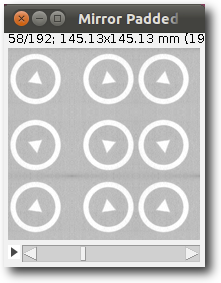
\includegraphics[width=0.3\textwidth]{Images/ToITKSolution_shadow}
\end{center}
\end{frame}


\subsection{Interface with OpenCV}
\begin{frame}[fragile]
\frametitle{To OpenCV}
Problem: Use SimpleITK from another image processing library (OpenCV)

\texttt{./ToOpenCV input.png output.png}

Steps:
\begin{itemize}
\item Load image using SimpleITK
\item Convert to OpenCV
\item Filter using OpenCV
\item Save using OpenCV
\end{itemize}
\end{frame}


\begin{frame}[fragile]
\frametitle{ToOpenCV}
Starting code: \texttt{ToOpenCV/ToOpenCV.cxx}\\
Directory: \texttt{SimpleITK-MICCAI-2011-Tutorial/Examples/AdvancedTutorial}
\begin{lstlisting}
#include <SimpleITK.h>
#include <opencv2/opencv.hpp>
namespace sitk = itk::simple;
...
  sitk::Image sitkImage = sitk::ReadImage ( inputFilename );

  // Convert SimpleITK to OpenCV image
  cv::Mat ocvImage;

  // Filter and write using OpenCV
  cv::Mat output;
  cv::medianBlur ( ocvImage, output, 5 );

  cv::imwrite ( outputFilename, output );
...
\end{lstlisting}
\end{frame}

\begin{frame}[fragile]
\frametitle{ToOpenCV -- Step 1}
Convert the SimpleITK image to a float
\begin{lstlisting}
  if ( sitkImage.GetPixelIDValue() != sitk::sitkFloat32 )
    {
    std::cout << "Input image is " << sitkImage.GetPixelIDTypeAsString()
              << " converting to float" << std::endl;
    sitkImage = sitk::Cast ( sitkImage, sitk::sitkFloat32 );
    }
\end{lstlisting}
\end{frame}

\begin{frame}[fragile]
\frametitle{ToOpenCV -- Step 2}
Get SimpleITK pixel data
\begin{lstlisting}
  // Convert SimpleITK to OpenCV image
  cv::Mat ocvImage ( sitkImage.GetHeight(), sitkImage.GetWidth(), CV_32F,
                     (void*)sitkImage.GetBufferAsFloat() );
\end{lstlisting}
\end{frame}

\begin{frame}[fragile]
\frametitle{ToOpenCV -- Step 3 (Optional)}
Display the before and after
\lstcppa
\begin{lstlisting}
// NB: the imshow function requires 8-bit data, so convert
cv::Mat temp;
ocvImage.convertTo ( temp, CV_8U );
cv::imshow ( "original slice", temp );
output.convertTo ( temp, CV_8U );
cv::imshow ( "bilateral filtering", temp );

std::cout << "Press any key to continue" << std::endl;
cv::waitKey();
\end{lstlisting}
\end{frame}

\begin{frame}[fragile]
\frametitle{To OpenCV Solution}
\texttt{\textasciitilde/Source/AdvancedTutorial-build/ToOpenCV/ToOpenCV \textbackslash \\
  \textasciitilde/Source/SimpleITK/Testing/Data/Input/cthead1.png \textbackslash \\
/tmp/head.png}
\begin{center}
  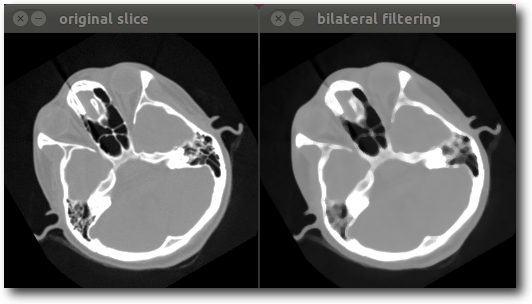
\includegraphics[width=0.5\textwidth]{Images/ToOpenCVSolution_shadow}
\end{center}
\end{frame}


\begin{frame}[fragile]
\frametitle{To OpenCV and Back}
Problem: Use OpenCV to process a SimpleITK volume slice-by-slice

\texttt{./ToOpenCVAndBack input.nii output.nii}

Steps:
\begin{itemize}
\item Load image using SimpleITK
\item Extract slice
\item Convert to OpenCV
\item Filter using OpenCV
\item Past slice back to SimpleITK
\item Save result
\end{itemize}
\end{frame}


\begin{frame}[fragile]
\frametitle{To OpenCV and Back}
Starting code: \texttt{ToOpenCVAndBack/ToOpenCVAndBack.cxx}\\
Directory: \texttt{SimpleITK-MICCAI-2011-Tutorial/Examples/AdvancedTutorial}
\begin{lstlisting}
namespace sitk = itk::simple;
...
sitk::Image sitkImage = sitk::ReadImage ( inputFilename );

for ( unsigned int s = 0; s < sitkImage.GetDepth(); s++ )
  {
  // Extract a slice
  // Go through ITK to grab the data
  // Convert ITK to OpenCV image
  // Filter using OpenCV
  // Convert back to SimpleITK
  // Paste the image back into SimpleITK
  }
sitk::WriteImage ( sOutput, outputFilename );
\end{lstlisting}
\end{frame}

\begin{frame}[fragile]
\frametitle{To OpenCV and Back - Step 1: Extract a slice}
\begin{lstlisting}
// Extract a slice
std::vector<unsigned int> size = sitkImage.GetSize();
size[2] = 1;
std::vector<int> index ( 3, 0 );
index[2] = s;
std::cout << "Extracting: " << s << std::endl;
sitk::Image slice = sitk::RegionOfInterest ( sitkImage, size, index );

if ( slice.GetPixelIDValue() != sitk::sitkFloat32 )
  {
  slice = sitk::Cast ( slice, sitk::sitkFloat32 );
  }
\end{lstlisting}
\end{frame}

\begin{frame}[fragile]
\frametitle{To OpenCV and Back - Step 2: Convert to OpenCV}
\begin{lstlisting}
// Convert ITK to OpenCV image
  cv::Mat ocvImage ( slice.GetHeight(), slice.GetWidth(),
                     CV_32F, (void*)sitkImage.GetBufferAsFloat() );
\end{lstlisting}
\end{frame}

\begin{frame}[fragile]
\frametitle{To OpenCV and Back - Step 3: Filter using OpenCV}
\begin{lstlisting}
  // Filter using OpenCV
  cv::Mat output;
  cv::Sobel ( ocvImage, output, -1, 1, 1 );
\end{lstlisting}
\end{frame}

\begin{frame}[fragile]
\frametitle{To OpenCV and Back - Step 4: Back to SimpleITK}
\begin{lstlisting}
  // Convert back to SimpleITK
  sitk::ImportImageFilter importer;
  importer.SetSize ( size );
  importer.SetSpacing ( sitkImage.GetSpacing() );
  importer.SetOrigin ( sitkImage.GetOrigin() );
  importer.SetBufferAsFloat ( output.ptr<float>() );

  sitk::Image toSimpleITKImage = importer.Execute();
\end{lstlisting}
\end{frame}

\begin{frame}[fragile]
\frametitle{To OpenCV and Back - Step 5: Paste back into SimpleITK volume}
\begin{lstlisting}
  // Paste the image back into SimpleITK
  // Paste ( Destination, Source, SourceSize, SourceIndex, DestIndex )
  sOutput = sitk::Paste ( sOutput, toSimpleITKImage,
            toSimpleITKImage.GetSize(), std::vector<int> ( 3,0 ), index );
\end{lstlisting}
\end{frame}

\begin{frame}[fragile]
\frametitle{To OpenCV and Back -- (Optional) Step 6: Show}
\begin{lstlisting}
  // (Optional) Show the results
  sitk::Show ( sOutput );
\end{lstlisting}
\end{frame}

\begin{frame}[fragile]
\frametitle{To OpenCV and Back Solution}
\texttt{\textasciitilde/Source/AdvancedTutorial-build/\textbackslash\\
ToOpenCVAndBack/ToOpenCVAndBack \textbackslash \\
  \textasciitilde/Source/SimpleITK/Testing/Data/Input/RA-Float.nrrd \textbackslash \\
  /tmp/foo.nii}
\begin{center}
  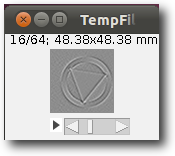
\includegraphics[width=0.4\textwidth]{Images/ToOpenCVAndBackSolution_shadow}
\end{center}
\end{frame}


\subsection{Java/Groovy}

\begin{frame}{Java/Groovy}
\fontsize{36pt}{36pt}\selectfont
\center
\begin{center}
Using SimpleITK from Java/Groovy
\end{center}
\vspace{20pt}
\begin{center}
\fontsize{11pt}{11pt}\selectfont
\texttt{Examples/AdvancedTutorial/Java/Example.groovy}
\end{center}
\end{frame}

\begin{frame}{Groovy}
\begin{itemize}
  \item Language build on Java
  \item Superset of Java
  \item Can be used interactively
\end{itemize}
\end{frame}

\begin{frame}[fragile]
\frametitle{Groovy}
\lstjava
\begin{lstlisting}
import org.itk.simple.*;

Image i;
i = new Image ( 64, 64, 64, PixelIDValueEnum.sitkInt16 );
SimpleITK.show ( i, "Blank" );
\end{lstlisting}
\fontsize{8pt}{8pt}\selectfont
\texttt{groovysh -classpath
 ./SimpleITK-Build/SimpleITK-Build/Wrapping/org.itk.simple.jar}
\end{frame}

\subsection{Other languages}

\begin{frame}{Quick Examples from Other Languages}
\fontsize{36pt}{36pt}\selectfont
\center
\begin{center}
Simple Gaussian in 8 languages
\end{center}
\vspace{20pt}
\begin{center}
\fontsize{11pt}{11pt}\selectfont
\texttt{AdvancedTutorial/SimpleGaussian/SimpleGaussian.*}
\end{center}
\end{frame}

\begin{frame}[fragile]
\frametitle{C++}
\lstcpp
\lstset{basicstyle={\ttfamily\tiny}}
\lstinputlisting{../Examples/AdvancedTutorial/SimpleGaussian/SimpleGaussian.cxx}
\end{frame}

\begin{frame}[fragile]
\lstcpp
\lstset{language=Ruby}
\frametitle{Ruby}
\lstinputlisting{../Examples/AdvancedTutorial/SimpleGaussian/SimpleGaussian.rb}
\end{frame}

\begin{frame}[fragile]
\lstcpp
\lstset{language=R}
\frametitle{R}
\lstinputlisting{../Examples/AdvancedTutorial/SimpleGaussian/SimpleGaussian.R}
\end{frame}

\begin{frame}[fragile]
\lstcpp
\lstset{language=Java}
\frametitle{C\#}
\lstinputlisting{../Examples/AdvancedTutorial/SimpleGaussian/SimpleGaussian.cs}
\end{frame}

\begin{frame}[fragile]
\lstcpp
\lstset{language=Java}
\frametitle{Java}
\lstinputlisting{../Examples/AdvancedTutorial/SimpleGaussian/SimpleGaussian.java}
\end{frame}

\begin{frame}[fragile]
\lstcpp
\lstset{language=Lua}
\frametitle{Lua}
\lstinputlisting{../Examples/AdvancedTutorial/SimpleGaussian/SimpleGaussian.lua}
\end{frame}

\begin{frame}[fragile]
\lstcpp
\lstset{language=Python}
\frametitle{Python}
\lstinputlisting{../Examples/AdvancedTutorial/SimpleGaussian/SimpleGaussian.py}
\end{frame}

\begin{frame}[fragile]
\lstcpp
\lstset{language=Tcl}
\frametitle{Tcl}
\lstinputlisting{../Examples/AdvancedTutorial/SimpleGaussian/SimpleGaussian.tcl}
\end{frame}

%% \section{Conclusion}

\begin{frame}{Conclusion}
\fontsize{36pt}{36pt}\selectfont
\center
\begin{center}
Conclusion
\end{center}
\end{frame}

\begin{frame}
\frametitle{Wrap-up}
\begin{itemize}
  \item Gentle introduction to ITK
  \item Introduce SimpleITK
  \item Provide hands-on experience
  \item Problem solving, not direction following
\end{itemize}
\end{frame}

\begin{frame}
\frametitle{Where to go next}
Some resources for using and extending SimpleITK
\small
\begin{itemize}
  \item Home Page
  	\begin{itemize} \item \url{http://www.simpleitk.org} \end{itemize}
  \item Documentation
  	\begin{itemize} \item \url{http://www.itk.org/SimpleITKDoxygen/html/} \end{itemize}
  \item Conventions
  	\begin{itemize} \item \url{http://www.itk.org/SimpleITKDoxygen/html/Conventions.html} \end{itemize}
  \item Contributions
  	\begin{itemize} \item \url{http://www.itk.org/SimpleITKDoxygen/html/Developer.html} \end{itemize}
\end{itemize}
\normalsize
\end{frame}



\begin{frame}
\frametitle{Wrap-up}
\end{frame}


\end{document}
